\section{Labeled Transition Systems}\label{sec:lts}

We make extensive use of the general theory of labeled transition
systems, a semantics approach especially relevant to communicating
concurrent systems.  As we are formalizing processors for
Turing-complete machine languages, it is challenging to prove that a
system preserves almost any aspect of processor behavior from a model
like SC.  To focus our theorems, we pick the time-honored property of
\emph{termination}.  An optimized system should terminate or diverge
iff the reference system could also terminate or diverge,
respectively.  All sorts of other interesting program properties are
reducible to this one, in the style of computability theory.
Our basic definitions of transition systems build in
special treatment of halting, so that we need not mention it
explicitly in most contexts to come.

\begin{defn}
A \textbf{labeled transition system (LTS)} is a ternary relation, over
$\mathcal S^H \times \mathcal L^\epsilon \times \mathcal S^H$, for some sets
$\mathcal S$ of states and $\mathcal L$ of labels. We usually do not mention
these sets explicitly, as they tend to be clear from context. We write
$X^\epsilon$ for lifting of a set $X$ to have an extra ``empty'' element
$\epsilon$ (like an \texttt{option} type in ML). We write $X^H$ for lifting of
a set $X$ to have an extra ``halt'' element $H$. We also implicitly consider
each LTS to be associated with an \emph{initial} state in $\mathcal S$.
\end{defn}

For LTS $A$, we write $\io{A}{s}{s'}{\ell}$ as shorthand for $(s,
\ell, s') \in A$, and we write $A_0$ for $A$'s initial state. The
intuition is that $A$ is one process within a concurrent system. The
label $\ell$ from set $\mathcal L$ of labels is produced when $A$
participates in some IO exchange with another process; otherwise it is
an empty or ``silent'' label $\epsilon$.  As a shorthand, we sometimes
omit labels for $\epsilon$ steps.

\subsection{Basic Constructions on LTSes}

From an LTS representing single-step system evolution, we can build %often want to build
an LTS capturing arbitrary-length evolutions.

\begin{defn}
The \textbf{transitive-reflexive closure} of $A$, written $A^{*}$, is a derived
LTS.  Where $A$'s states and labels are $\mathcal S$ and $\mathcal L$, the
states of $A^{*}$ are $\mathcal S$, and the labels are $\mathcal L^{*}$, or
\emph{sequences} of labels from the original system.  $A^{*}$ steps from $s$ to
$s'$ when there exist zero or more transitions in $A$ that move from $s$ to
$s'$.  The label of this transition is the \emph{concatenation} of all labels
generated in $A$, where the empty or ``silent'' label $\epsilon$ is treated as
an identity element for concatenation.
\end{defn}

We also want to compose $n$ copies of an LTS together, with no explicit
communication between them.  We apply this construction later to lift a
single-CPU system to a multi-CPU system.

\begin{defn}
The \textbf{$n$-repetition} of $A$, written $\smulti{n}{A}$, is a derived LTS.
Where $A$'s states and labels are $\mathcal S$ and $\mathcal L$, the states of
$\smulti{n}{A}$ are $\mathcal S^n$, and the labels are $[1, n] \times \mathcal
L$, or pairs that \emph{tag} labels with which component system generated them.
These labels are generated only when the component system generates a label.
The whole system halts whenever one of the components halts.  We define the
transition relation with the following inference rules. We treat $n$-tuples as
functions keyed on numeric positions, and we write $\theta[i := v]$ for
updating $n$-tuple $\theta$ to overwrite the $i$th position with value $v$, and
we treat any label $(i, \epsilon)$ as $\epsilon$.
\small
$$\inference[i]
{\theta(i) = a & \io{$A$}{a}{a'}{\ell} & a' \neq H}
{\io{$\smulti{n}{A}$}{\theta}{\theta[i:=a']}{i,\ell}}
\quad \inference[H]
{\io{$A$}{\theta(i)}{H}{\ell}}
{\io{$\smulti{n}{A}$}{\theta}{H}{i,\ell}}
$$
\end{defn}

Eventually, we need processes to be able to communicate with each
other, which we formalize via the $+$ composition operator. It
connects same-label transitions in the two systems, treating the label
as a cooperative communication event that may now be hidden from the
outside world, as an $\epsilon$ label.

\begin{defn}\label{plus}
Where $A$ and $B$ are two LTSes sharing labels set $\mathcal L$,
and with state sets $\mathcal S_A$ and
$\mathcal S_B$ respectively, the \textbf{communicating composition} $A + B$ is
a new LTS with states $\mathcal S_A \times \mathcal S_B$ and an empty label set,
defined as follows:
\vspace{-.2in}\begin{center}
\small
$$\inference[$A$]
{\io{$A$}{a}{a'}{} & a' \neq H}
{\io{$A + B$}{a, b}{a', b}{}}
\quad \inference[$B$]
{\io{$B$}{b}{b'}{} & b' \neq H}
{\io{$A + B$}{a, b}{a, b'}{}}$$
$$\inference[H$_A$]
{\io{$A$}{a}{H}{}}
{\io{$A + B$}{a, b}{H}{}}
\quad \inference[H$_B$]
{\io{$B$}{b}{H}{}}
{\io{$A + B$}{a, b}{H}{}}$$
$$\inference[Join]
{\io{$A$}{a}{a'}{\ell} & \io{$B$}{b}{b'}{\ell} & a', b' \neq H}
{\io{$A + B$}{a, b}{a', b'}{}}$$
\end{center}
\end{defn}

\subsection{Refinement Between LTSes}

We need a notion of when one LTS ``implements'' another.  Intuitively,
transition labels and halting are all that the outside world
can observe. Two systems that produce identical labels and termination behavior
under all circumstances can be considered as safe substitutes for
one another. We will only need an asymmetrical notion of compatibility:

\begin{defn}\label{refines}
For some label domain $\mathcal L$, let $f : \mathcal L \to \mathcal L^\epsilon$ 
be a function that is able to replace labels with alternative
labels, or erase them altogether. Let LTSes $A$ and $B$ have the same label
set $\mathcal L$. We say that
\textbf{$A$ trace-refines $B$ w.r.t. $f$}, or $A \sqsubseteq_f B$, if:
\begin{multline*}
\forall s_A, \eta. \; \io{$A^{*}$}{A_0}{s_A}{\eta} \Rightarrow \exists s_B. \;
\io{$B^{*}$}{B_0}{s_B}{f(\eta)} \; \wedge \\
(s_A = H \Leftrightarrow s_B = H)
\end{multline*}
Each label in the trace is replaced by the mapping of $f$ on it, and
labels mapped to $\epsilon$ by $f$ are dropped. $f$ is overloaded
to denote that multilabel version when applied to $\eta$.
\end{defn}

As a shorthand, we write $A \sqsubseteq B$ for $A \sqsubseteq_\mathsf{id} B$,
for $\mathsf{id}$ an identity function, forcing traces in the two systems to
match exactly. Under this notion of identical traces, we say that $A$
is sound w.r.t. $B$.

\subsection{A Few Useful Lemmas}

The reflexivity and transitivity properties of refinement are crucial to help us
structure modular proofs.

\begin{theorem}\label{transitive}
$\sqsubseteq$ is reflexive and transitive.
\end{theorem}

Another crucial proof step is to lift a single-process result to the $n$-way
replication of that process.

\begin{theorem}\label{liftn}
If $A \sqsubseteq_f B$, then $\smulti{n}{A} \sqsubseteq_{f^n} \smulti{n}{B}$, where
$f^n$ is $f$ lifted appropriately to deal with indices ($f^n(i, \ell) =
(i, \ell')$ when $f(\ell) = \ell'$, and $f^n(i, \ell) = \epsilon$ when
$f(\ell) = \epsilon$).
\end{theorem}

We will also need a result applying to communicating compositions.

\begin{theorem}\label{liftplus}
If $A \sqsubseteq_f A'$ and $B \sqsubseteq_f B'$, then $A + B \sqsubseteq A' +
B'$. In other words, if systems $A$ and $B$ are individually simulated by $A'$ and
$B'$ on identical alteration of the traces, then the composed
system $A+B$ will be sound with respect to $A'+B'$.
\end{theorem}

%\begin{figure}
%\small
%\centering
%\begin{boxedminipage}[c]{.48\textwidth}
%%\centering
%\inference
%[Halt]
%{\theta(i) = (s, \pc) & \dec(s,\pc) = H}
%{\io{SC}{\theta,m}{H}{}}
%
%\inference
%[NonMem]
%{\theta(i) = (s, \pc) & \dec(s,\pc) = (\nm, x) \\ \exec(s, \pc, (\nm, x)) = (\pc', s')}
%{\io{SC}{\theta,m}{\theta[i \coloneqq (s', \pc')], m}{}}
%
%\inference
%[Load]
%{\theta(i) = (s,\pc) & \dec(s,\pc) = (\ld, x, a) \\ \exec(s, \pc, (\ld, x, m(a))) = (\pc', s')}
%{\io{SC}{\theta,m}{\theta[i\coloneqq(s',\pc')],m}{}}
%
%\inference
%[Store]
%{\theta(i) = (s,\pc) & \dec(s,\pc) = (\st, a, v) \\ \exec(s, \pc, (\st)) = (\pc', s')}
%{\io{SC}{\theta,m}{\theta[i\coloneqq(s',\pc')],m[a\coloneqq v]}{}}
%\end{boxedminipage}
%\caption{LTS for sequential consistency with $n$ simple processors}
%\label{Ref}
%\end{figure}
%
%It is worth noting that the LTS notation described above, along with the
%composition operators are very similar to the semantics of hardware designs
%written in Bluespec. As an example consider an inference rule in LTS and the
%corresponding code in Bluespec in Figure \ref{both}. This code was actually
%written for the PowerPC system \cite{Khan:PowerPc} (we will be using this rule
%later in the paper when we describe the coherent caches).
\section{Decomposing a Shared-Memory Multiprocessor System}
\label{sec:store-atomicity}

\begin{figure}
\centering
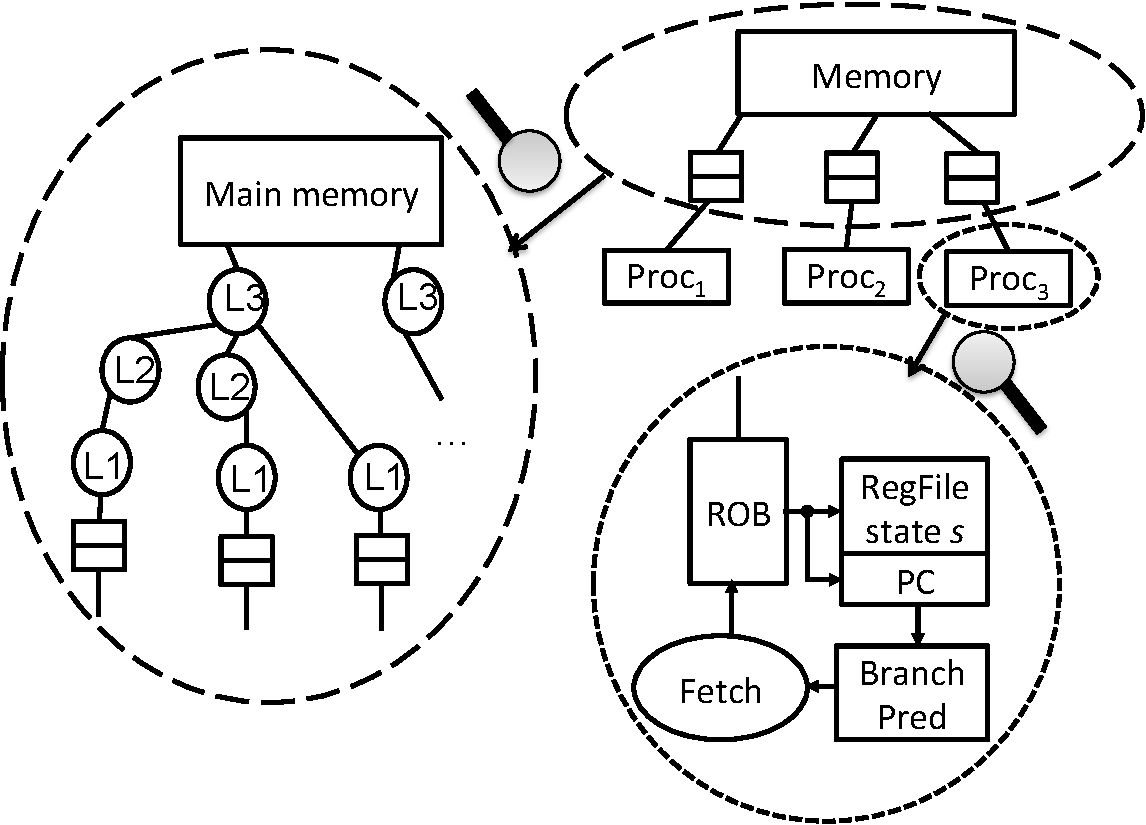
\includegraphics[scale=.43]{zoom}
\caption{Components of a multiprocessor system}
\label{zoom}
\end{figure}

Any conventional multiprocessor system can be divided logically into 3 components as shown in Figure \ref{zoom}. 
The top-level system design is shown at top right, while the details of its components, the memory system and the processor ($P_i$), are shown in the magnified boxes. The processor component $P_i$ can be implemented in a variety of ways, from one executing instructions one-by-one in program order, to a complex one speculatively executing many instructions concurrently to exploit parallelism. The memory component is normally implemented using a hierarchy of caches, in order to increase the performance of the overall system, since the latency of accessing memory directly is large compared to that of accessing a much smaller cache. The component between each processor and the global memory subsystem contains local load/store buffers, $B_i$, each specific to a processor $P_i$. 

%\begin{figure}
%\small
%\centering
%\begin{boxedminipage}[c]{.48\textwidth}
%\inference
%[Load]
%{}
%{\io{$M_m$}{m}{m}{p, ((\ld\req,a),(\ld\resp,m(a)), \_)}}
%
%\inference
%[Store]
%{}
%{\io{$M_m$}{m}{m[a\coloneqq v]}{p, (\st, a, v)}}
%
%\end{boxedminipage}
%\caption{LTS for a simple memory}
%\label{M_m}
%\end{figure}

Popular instruction set architectures, such as Intel x86, ARM, and PowerPC, do not guarantee sequential consistency.  That is, their behavior makes it unsound to imagine that
the different processors of a shared-memory system are running
according to simple interleaving of instructions, where each instruction executes atomically.  However, we want to emphasize that, in every weak-memory system we are aware of, \emph{the main memory still exposes atomic loads and stores}!  The weaker semantics arises only because of (1)
reordering of memory instructions by the core $P_i$ and/or (2) the
properties of the local buffers $B_i$ connected to each processor
$P_i$.  For instance, if $B_i$ were a store buffer, into which the
committed stores from an in-order processor $P_i$ are enqueued, and if
any ``subsequent'' load from the same processor $P_i$ is allowed to read and commit the latest value from the store buffer, then such a multiprocessor system is said to implement the TSO~\cite{x86tsocacm10} memory
model. 

\begin{figure}
\small
\centering
\begin{boxedminipage}[c]{.48\textwidth}
\inference
[Ins]
{}
{\iorn{$M_m$}{\inp, \outp, m}{\inp[p \coloneqq \{q\} \uplus \inp(p)], \outp, m}{p}{q}}

\inference
[Rm]
{\outp(p) = \mathit{rs} \uplus \{r\}}
{\ioln{$M_m$}{\inp, \outp, m}{\inp, \outp[p \coloneqq \mathit{rs}], m}{p}{r}}

\inference
[Ld]
{\inp(p) = \mathit{qs} \uplus \{t, \ld,a\}}
{\ioxe{$M_m$}{\inp, \\\outp, m}{\inp[p \coloneqq \mathit{qs}], \outp[p \coloneqq\\
\;\;\;(t, \ld, m(a)) \uplus \outp(p)], m}{}}

\inference
[St]
{\inp(p) = \mathit{qs} \uplus \{\st,a,v\}}
{\ioxe{$M_m$}{\inp, \\\outp, m}{\inp[p \coloneqq \mathit{qs}], \outp[p \coloneqq
(\st) \\\;\;\;\uplus \outp(p)], m[a\coloneqq v]}{}}%p, (\st, a,v)}}

\end{boxedminipage}
\caption{LTS for a simple memory}
\label{$M_m$}
\end{figure}

So, we focus on this opportunity to simplify proof decomposition.  We will
prove that our main memory component satisfies an intuitive \emph{store
atomicity} property.  Despite the potential red herring of the word
``atomicity,'' this specification is appropriate even for implementation of
weaker memory models than SC.  Store atomicity can be understood via the
operational semantics of Figure \ref{$M_m$}, describing an LTS that receives
load and store requests ($\ld$ and $\st$) from processors and sends back load
responses ($\ld\resp$). The transfer happens via input buffers $\inp(p)$ from
processor $p$ and output buffers $\outp(p)$ to processor $p$.  Note that this
model allows the memory system to answer pending memory requests in any order,
even potentially reordering requests from a single processor,
so long as, whenever it does process a request, that action appears to take
place \emph{atomically}.

The memory component is composed of a \emph{hierarchy of caches}, where each
cache node (labeled like ``L1,'' ``L2,'' etc.) communicates only with its
neighbors in the graph.  Each processor has a dedicated L1 cache, from which we
do our best to satisfy all memory requests, to avoid the latency of a
round-trip with main memory.  With an L1 cache miss, we may still find a hit in
a parent cache below the level of main memory, realizing a smaller but still
significant speedup.  Therefore it is the responsibility of the hierarchy of
caches, which forms the memory subcomponent, to implement the store atomicity
property. In fact, as we will prove in Section \ref{sec:cc}, the purpose of the
cache-coherence protocol is to establish this invariant for the memory
subcomponent.  Concretely, we have verified a \emph{directory-based} protocol
for coordinating an arbitrary tree of caches, where each node stores a
conservative approximation of its children's states.

As an instance of the above decomposition, we will prove that a multiprocessor
system with no local buffering in between the processor and the memory
components indeed implements sequential consistency. We implement a highly
speculative processor that executes instructions and issues loads out of order,
but commits instructions (once some ``verification'' is done) in order. This idea
of verification loads for a speculative processor is not new \cite{cain}.

The processor itself can be decomposed into several components. In the
zoomed-in version of Figure \ref{zoom}, we show a highly speculative,
out-of-order issue processor. We have the normal architectural state, such as
values of registers.  Our proofs are generic over \emph{a family of instruction
set architectures}, with parameters for opcode sets and functions for executing
opcodes and decoding them from memory.  Other key components are a \emph{branch
predictor}, which guesses at the control-flow path that a processor will
follow, to facilitate speculation; and a \emph{reorder buffer (ROB)}, which
decides which instructions along that path to try executing ahead of schedule.
Our proofs apply to an arbitrary branch predictor, and they work for any
reorder buffer satisfying a simple semantic condition.


Our framework establishes theorems of the form ``if system $A$ has a run with
some particular observable behavior, then system $B$ also has a run with the
same behavior.''  In this sense, we say that $A$ correctly implements $B$.
Other important properties, such as \emph{deadlock freedom} for $A$ (which
might get stuck without producing any useful behavior), we leave for future
work.

\section{Specifying Sequential Consistency}\label{sec:sc}

\begin{figure}
\small
\centering
\begin{boxedminipage}[c]{.48\textwidth}
%\centering
\inference
[Halt]
{\theta(i) = (s, \pc) & \dec(s,\pc) = H}
{\io{SC}{\theta,m}{H}{}}

\inference
[NonMem]
{\theta(i) = (s, \pc) & \dec(s,\pc) = (\nm, x) \\ \exec(s, \pc, (\nm, x)) = (s',\pc')}
{\io{SC}{\theta,m}{\theta[i \coloneqq (s', \pc')], m}{}}

\inference
[Load]
{\theta(i) = (s,\pc) & \dec(s,\pc) = (\ld, x, a) \\ \exec(s, \pc, (\ld, x, m(a))) = (s',\pc')}
{\io{SC}{\theta,m}{\theta[i\coloneqq(s',\pc')],m}{}}

\inference
[Store]
{\theta(i) = (s,\pc) & \dec(s,\pc) = (\st, a, v) \\ \exec(s, \pc, (\st)) = (s',\pc')}
{\io{SC}{\theta,m}{\theta[i\coloneqq(s',\pc')],m[a\coloneqq v]}{}}
\end{boxedminipage}
\caption{LTS for SC with $n$ simple processors}
\label{Ref}
\end{figure}

Our final theorem in this paper establishes that a particular complex hardware
system implements sequential consistency (SC) properly.  We state the theorem
in terms of the trace refinement relation $\sqsubseteq$ developed in the prior
section.  Therefore, we need to define an LTS embodying SC.  The simpler this
system, the better.  We do not need to worry about its performance properties,
since we will prove that an optimized system remains faithful to it.

Figure~\ref{Ref} defines an $n$-processor, sequentially consistent system as an
LTS.  The definition is parametrized over details of an \emph{instruction set
architecture} (ISA).  In particular, the ISA gives us some domains of
architectural states $s$ (e.g., register files) and of program counters $\pc$.
A function $\dec(s, \pc)$ figures out which instruction $\pc$ references in the
current state, returning the instruction's ``decoded'' form.  A companion
function $\exec(s, \pc, \mathit{dec})$ actually executes the instruction,
returning the new state $s'$ and the next program counter $\pc'$.

The legal instruction forms, which are outputs of $\dec$, are $(\nm, x)$, for
an operation not accessing memory; $(\ld, x, a)$, for a memory load from
address $a$; $(\st, a, v)$, for a memory store of value $v$ to address $a$; and
$H$, for a ``halt'' instruction that moves the LTS to state $H$. The parameter
$x$ above represents the rest of the instruction, including the
opcode, registers, constants, \etc{}

The legal inputs to $\exec$ encode both a decoded instruction and any relevant
responses from the memory system.  These inputs are $(\nm, x)$ and $\st$, which
need no extra input from the memory; and $(\ld, x, v)$, where $v$ gives the
contents of the requested memory cell.

We define the initial state of SC as $(\theta_0, m_0)$, where $m_0$ is
some initial memory fixed throughout our development, mapping every
address to value $v_0$; and $\theta_0$ maps every processor ID to
$(s_0, \pc_0)$, using architecture-specific default values $s_0$ and
$\pc_0$.

\medskip

This LTS encodes Lamport's notion of SC, where processors take turns executing
nondeterministically in a simple interleaving.  We need know very few details
of the ISA to define the SC model.  Our final, optimized system is parametrized
over an ISA in the same way.  In the course of the rest of this paper, we will
define an optimized system $O$ and prove $O \sqsubseteq \text{SC}$.

However, we are not interested merely in verifying the particular system $O$.
Instead, we want to structure our proof \emph{modularly}, so that different
common hardware components can be verified separately, and, in a black-box
manner, we may assemble a correctness proof for any composition of these
components.  For instance, we want to verify CPUs and memory systems
separately, picking any realization of each to produce a verified system, with
minimal new proof effort. As a more concrete example, memory systems should be
verifiable independently of which weak memory model processors assume; we want
to reuse memory proofs for different kinds of processors.

To support this style of modular decomposition, we need to introduce a few
intermediate systems.

Note that, in this setting, an operational specification like the LTS
for SC is precisely the right characterization of \emph{full functional
  correctness} for a hardware design, much as a
precondition-postcondition pair does that job in a partial-correctness
Hoare logic.  Our SC LTS fully constrains observable behavior of a
system to remain consistent with simple interleaving.  Similar
operational models are possible as top-level specifications for
systems following weaker memory models, by giving the LTS for the \emph{Local
Buffer} component and composing the three components simultaneously.

\begin{figure}
\small
\centering
\begin{boxedminipage}[c]{.48\textwidth}
\inference
[Halt]
{\dec(s,\pc) = H}
{\io{P$_\text{ref}$}{s,\pc,\bot}{H}{}}

\inference
[NM]
{\dec(s,\pc) = (\nm, x) & \exec(s, \pc, (\nm, x)) = (s', \pc')}
{\ioe{P$_\text{ref}$}{s,\pc,\bot}{s', \pc', \bot}}

\inference
[LdRq]
{\dec(s,\pc) = (\ld, x, a)}
{\ior{P$_\text{ref}$}{s, \pc, \bot}
{s, \pc, \top}{\epsilon, \ld, a}}

\inference
[StRq]
{\dec(s,\pc) = (\st, a, v)}
{\ior{P$_\text{ref}$}{s, \pc, \bot}
{s, \pc, \top}{\st, a, v}}

\inference
[LdRp]
{\dec(s,\pc) = (\ld, x, a) & \exec(s, \pc, (\ld, x, v)) = (s',\pc')}
{\iol{P$_\text{ref}$}{s, \pc, \top}
{s', \pc', \bot}{\epsilon, \ld, v}}

\inference
[StRp]
{\dec(s,\pc) = (\st, a, v) & \exec(s, \pc, (\st)) = (s',\pc')}
{\iol{P$_\text{ref}$}{s, \pc, \top}
{s', \pc', \bot}{\st}}
\end{boxedminipage}

\caption{LTS for a simple decoupled processor (P$_{\text{ref}}$)}
\label{Pref$}
\end{figure}


\section{Respecifying Sequential Consistency with Communication}\label{sec:ref}

Realistic hardware systems do not implement the monolithic SC model of
Figure~\ref{Ref} directly.  Instead, there is usually a split between
processors and memory. Here we formalize that split using LTSes that 
compose to produce a system refining the simple SC model.

Figure~\ref{Pref$} defines an LTS for a simple \emph{decoupled} processor
(P$_\text{ref}$).  That is, memory does not appear within a processor's state, but
instead, to load from or store to an address, we send \emph{requests} to the
memory system and receive its \emph{responses}.  Both kinds of messages are
encoded as labels, $\text{ToM}$ for requests to memory and $\text{ToP}$ for
responses from memory back to the processor.

A state of P$_{\text{ref}}$ is a triple $(s, \pc, \wait)$, giving the current architectural
state $s$ and program counter $\pc$, as well as a Boolean flag $\wait$
indicating whether the processor is blocked waiting for a response from the
memory system. As in the SC model, we change the state of the processor to $H$
whenever $\dec$ returns $H$. 
%Note that there is some subtlety in the design of
%this semantics regarding halting; we plan ahead to be sure we will be able to prove the
%appropriate simulation facts.  Those proofs would be harder if, \eg{}
%a processor could halt while it is still waiting for a memory response.

As initial state for system $P_\text{ref}$, we use $(s_0, \pc_0, \bot)$.

%\medskip

The simple memory defined earlier in Figure~\ref{$M_m$} is meant to be composed with P$_{\text{ref}}$
processors.  %The input-output interface of this memory $M_m$ is largely what
%one would expect from the P$_{\text{ref}}$ definition. 
%However, in anticipation of the
%more complex processor we will define later, we add requests and responses for
%\emph{speculative loads}.  These are load operations that a processor may
a%ttempt, before it knows that the program will actually need the result.  Many
s%peculative loads from a single processor may be in flight at once, improving
p%erformance via parallelism. 
A request to memory like $(t, \ld, a)$ asks
for the value of memory cell $a$, associating a \emph{tag} $t$ that the
processor can use to match responses to requests.  Those responses take the
form $(t, \ld, v)$, giving the value $v$ of the requested memory address.

A memory state is a triple $(\inp, \outp, m)$, giving not just the
memory $m$ itself, but also buffers $\inp$ and $\outp$ for receiving
processor requests and batching up responses to processors,
respectively.  We define the initial state of the $M_m$ LTS as
$(\emptyset, \emptyset, m_0)$, with empty queues.

%Note that we have used $\uplus$ for inserting (or removing) from the buffers
%$\inp$ and $\outp$. The intent is to convey that $\inp$ and $\outp$ are treated
%as unordered sets. We will later use $\coloncolon$ for inserting (or removing)
%from FIFO buffers. Intuitively, the unordered requests/responses set suffices
%even for requests/responses for the same address because the processor always
%waits for a response before sending the next request.
%\medskip

Now we can compose these LTSes to produce an implementation of SC. 
% Rule SpLoad
%in Figure~\ref{$M_m$} will be irrelevant in this particular composition, since
%P$_{\text{ref}}$ never does speculation.

For a system of $n$ processors, our decoupled SC implementation is
$\text{P$^n_{\text{ref}}$} + M_m$.

\begin{figure}[h]
\begin{boxedminipage}{\columnwidth}
\small
$\upd((s, \pc, \_), \mathit{rs}) =$

\begin{math}
\;\;\;\;\;\left\{
\begin{array}{ll}
s', \pc' &: (\ld, v) \in \mathit{rs} \wedge \dec(s, \pc) = (\ld, x, a) \wedge\\
\multicolumn{2}{r}{\exec(s, \pc, (\ld, x, v)) = (s',\pc'))}\\
s', \pc' &: (\st) \in \mathit{rs} \wedge \dec(s, \pc) = (\st, a, v) \wedge\\
\multicolumn{2}{r}{\exec(s, \pc, (\st)) = (s',\pc')}\\
s, \pc &: \text{otherwise if } \dec(pc,s) \neq H\\
H &: \text{otherwise}
\end{array}
\right.
\end{math}
\end{boxedminipage}
\caption{Mapping of states from $(\text{P$^n_\text{ref}$} + M_m)$ to SC}
\label{smap}
\end{figure}

\begin{theorem}
$\text{P$^n_{\text{ref}}$} + M_m \sqsubseteq SC$\label{scthm}
\end{theorem}
\begin{prf}
By induction on traces of the decoupled system.  We need to choose an
abstraction function $f$ from states of the complex system to states of
the simple system.  This function must be inductive in the
appropriate sense: a step from $s$ to $s'$ on the left of the
simulation relation must be matched by sequences of steps on the right
from $f(s)$ to $f(s')$.

Figure~\ref{smap} defines a suitable function $\upd$ applying to the
state of a single processor, and our abstraction function is the
natural lifting to $n$ processors.
The single-processor version $\upd$ maps
the decoupled state of a processor to an SC state, when also given the
set $rs$ of memory responses that have not been processed yet. If such a
response exists, then the updated $s', \pc'$ is the result of
receiving the response and performing the state updates on the current $s,
\pc$ pair.  We can also prove that multiple responses will not be present in
the $rs$ set at any point, intuitively because the processor goes into a wait
state as soon as it sends a request, and the single response, if present, will
correspond exactly to the instruction currently waiting for the response.
Therefore, the apparently ambiguous definition of $\upd$ is actually
well-founded.  The only interesting case in the proof arises when the memory adds a
response to $rs$; one has to show that the SC system can lead to the same
(projected) state.
\end{prf}

\paragraph{The final theorem and the proof plan:} 
In this section we divided a multiprocessor system into two rather simple
components, processor represented by $P_\text{ref}$ and memory represented by
$M_m$. In the following two sections we will develop more complex, optimized
versions of each piece and prove their correctness, that is, $P_\text{so}$, the
speculative out-of-order processor, is sound with respect to $P_\text{ref}$ and
$M_c$, the cache memory, is sound with respect to $M_m$. In proving the
soundness of $P_\text{so}$ with respect to $P_\text{ref}$, we need to focus
only on non-speculative communications. The main theorem we are after is to
show that P$^n_\text{so}+ M_c$ is SC, by showing that it is sound with respect
to P$^n_\text{ref}+ M_m$. Figure~\ref{proofs} gives the overall proof structure
that we will employ.


\begin{figure}
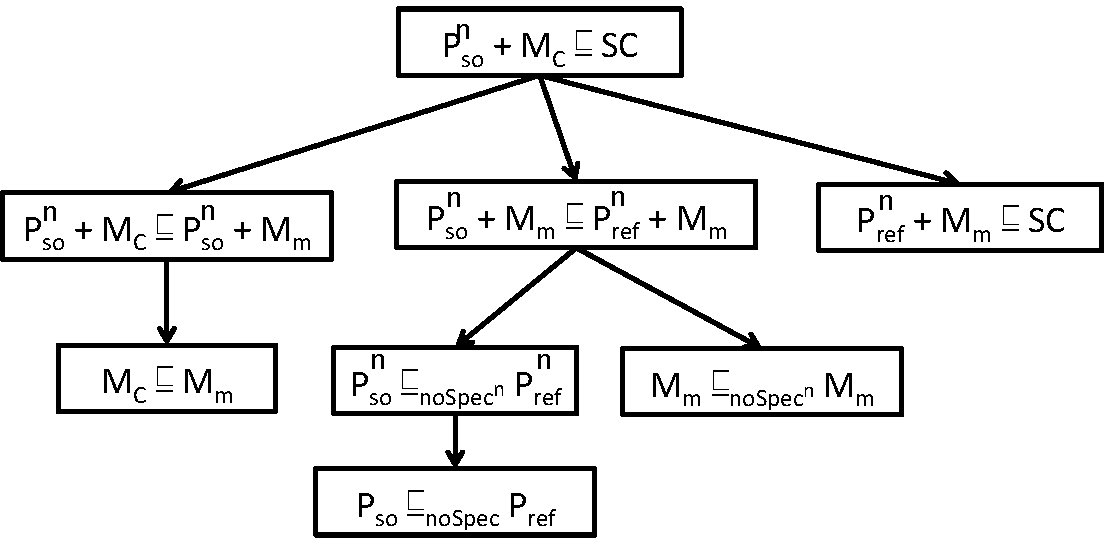
\includegraphics[scale=.45]{proofs}
\caption{Overall proof structure}
\label{proofs}
\end{figure}


\section{Speculative Out-Of-Order Processor}\label{sec:ooo}

We implement a \emph{speculative} processor, which may create many
simultaneous outstanding requests to the memory, as an optimization to
increase parallelism.  Our processor proof is in some sense generic
over correct speculation strategies.  We parametrize over two key
components of a processor design: a \emph{branch predictor}, which
makes guesses about processor-local control flow in advance of
%receiving enough memory responses to resolve
resolving conditional jumps; and a
\emph{reorder buffer}, which decides what speculative instructions (like memory loads)
are worth issuing at which moments (in effect \emph{reordering} later
instructions to happen before earlier instructions have finished).

The branch predictor is the simpler of the two components, whose state
is indicated with metavariable $\ppc$.
The operations on such state are $\curPpc(\ppc)$, to extract the
current program-counter prediction; $\nextPpc(\ppc)$, to get the predicted
program-counter for the next instruction; and $\setBp(\ppc, \pc)$,
to reset prediction to begin at a known-accurate position $\pc$. We need to impose no explicit correctness criterion on
branch predictors; the processor uses predictions only as hints, and
it always resets the predictor using $\setBp$ after detecting an
inaccurate hint.

The interface and formal contract of a reorder buffer are more
involved.  We write $\rob$ as a metavariable for reorder buffer
state. $\phi$ denotes the state of an empty buffer. The operations associated with $\rob$ are:
\begin{itemize}
%\item $\phi$, the state of an empty buffer.
\item $\add(\pc, \rob)$, which appends the program instruction at location $\pc$ to the list of instructions that the buffer is allowed to consider executing.
\item $\compute(\rob)$, which models a
step of computation inside the buffer, returning both an updated state
and an optional speculative load to issue. For instance, it invokes the $\dec$
and $\exec$ functions (as defined for SC) internally to obtain the next program
counter, state, \etc{} (but the actual states are not updated).
\item $\upd\ld(\rob,t,v)$, which informs the buffer that the memory
has returned result value $v$ for the speculative load with tag $t \neq \epsilon$.
\item $\commit(\rob)$, which returns the next instruction in serial
program order, if we have accumulated enough memory responses to execute it
accurately, or returns
$\epsilon$ otherwise.  When $\commit$ returns an instruction, it also
returns the associated program counter plus the next program counter
we would advance to afterward.
 Furthermore, the instruction is
extended with any relevant response from memory (used only for load
instructions, obtained through $\upd\ld$) and with the new architectural state (\eg{} register
file) after execution.
\item $\retire(\rob)$, which informs the buffer that its $\commit$
instruction was executed successfully, so it is time to move on to the
next instruction.
\end{itemize}

We postpone characterization of correct reorder buffers until after we
present the LTS for speculating processors.

\begin{figure}[t]
\small
\centering
\begin{boxedminipage}[c]{.95\textwidth}
\inference[Fetch]
{}
{\ioxe{P$_\text{so}$}{\hspace{-.2cm}s,\pc,\wait,\\\rob,\ppc}{\hspace{-.2cm}s,\pc,\wait,\add(\curPpc(\ppc),\\\;\;\;\rob),\nextPpc(\ppc)}}

\inference[Compute]
{\compute(\rob) = (\rob',\epsilon)}
{\ioe{\text{P$_\text{so}$}}{s,\pc,\wait,\rob,\ppc}{s,\pc,\wait,\rob',\ppc}}

\inference[SpLdRq]
{\compute(\rob) = (\rob',(\spc\ld,t,a))}
{\ior{\text{P$_\text{so}$}}{s,\pc,\wait,\rob,\ppc}{s,\pc,\wait,\rob',\ppc}
{t,\ld, a}}

\inference[SpLdRp]
{t \neq \epsilon}
{\iox{\text{P$_\text{so}$}}{s,\pc,\wait,\\\rob,\ppc}
{s,\pc,\wait,\\\upd\ld(\rob, t, v),\ppc
}{\text{ToP}(t,\ld,v)}}

\inference[Abort]
{\commit(\rob) = (\pc',\_,\_) & \pc' \neq \pc}
{\ioxe{\text{P$_\text{so}$}}{s,\pc,\wait,\\\rob,\ppc}{s,\pc,\wait,\phi,\\\setBp(\ppc,\pc)}}

\inference[Halt]
{\commit(\rob) = H}
{\ioe{\text{P$_\text{so}$}}{s,\pc,\bot,\rob,\ppc}{H}}

\inference[Nm]
{\commit(\rob) = (\pc,\pc',(\nm,s'))}
{\ioe{\text{P$_\text{so}$}}{s,\pc,\bot,\rob,\ppc}{s',\pc',\bot,\retire(\rob),\ppc}}

\inference[StRq]
{\commit(\rob) = (\pc,\pc',(\st,a,v,s'))}
{\ior{\text{P$_\text{so}$}}{s,\pc,\bot,\rob,\ppc}{s,\pc,\top,\rob,\ppc}
{\st, a, v}}

\inference[LdRq]
{\commit(\rob) = (\pc,\pc',(\ld,x,a,v,s'))}
{\ior{\text{P$_\text{so}$}}{s,\pc,\bot,\rob,\ppc}{s,\pc,\top,\rob,\ppc}{\epsilon, \ld, a}}
\inference[StRp]
{\commit(\rob) = (\pc,\pc',(\st,a,v,s'))}
{\iol{\text{P$_\text{so}$}}{s,\pc,\top,\rob,\ppc}{s',\pc',\bot,\retire(\rob),\ppc}{\st}}

\inference[LdRpGood]
{\commit(\rob) = (\pc,\pc',(\ld,x,a,v,s'))}
{\iox{\text{P$_\text{so}$}}{s,\pc,\top,\\\rob,\ppc}{s',\pc',\bot,\\\retire(\rob),\ppc}{\text{ToP}(\epsilon, \ld,v)}}

\inference[LdRpBad]
{\commit(\rob) = (\pc,\pc',(\ld,x,a,v',s')) \\ v' \neq v & \exec(s,\pc,(\ld,x,v)) = (s'',\pc'')}
{\iox{\text{P$_\text{so}$}}{s,\pc,\top,\\\rob,\ppc}{s'',\pc'',\bot,\phi,\\\setBp(\ppc,\pc)}{\text{ToP}(\epsilon, \ld, v)}}


\end{boxedminipage}

\caption{Speculating, out-of-order issue processor}
\label{Ooo}
\end{figure}

Figure~\ref{Ooo} defines that LTS,
P$_{\texttt{so}}$. This processor may issue arbitrary speculative
loads, but it only ever \emph{commits} the next instruction in serial
program order. 
We will see the processor issue two kinds of loads, a speculative
load (whose tag is not $\epsilon$) and a commit or real load (whose tag is $\epsilon$).  To maintain SC, every speculative
load must have a matching verification load later on, and we maintain
the illusion that the program only depends on the results of
verification loads, which, along with stores, \emph{must be issued in
serial program order}.

When committing a
previously issued speculative load instruction, the associated speculative
memory load response is verified against the new commit load response. If the
resulting values do not match, the processor terminates all past uncommitted
speculation, by emptying the reorder buffer and resetting the
next predicted program counter in the branch predictor to the correct next value. This step mimics
the mechanism implemented in most modern-day processors, operating on the
conservative assumption that the processor may have performed arbitrary
incorrect speculation after receiving the inaccurate response from
memory.  (Note that here ``inaccurate'' does not mean ``wrong at
the time the response was received,'' but rather ``wrong at commit
time'' or ``correct before, but not anymore.'')

A full processor state is $(s, \pc, \wait, \rob, \ppc)$, comprising
architectural state, the program counter, a Boolean flag indicating
whether the processor is waiting for a memory response about an
instruction being committed, and the reorder buffer and branch
predictor states. Its initial state is given by $(s_0, \pc_0, \bot, \phi, \ppc_0)$.
The interface of this processor with memory (\ie{}
communication labels with $\toM, \toP$) is identical
to that of the reference processor.
% but now we can exercise a memory
%system's transitions for speculative loads.

%The processor state is represented in the form $(s,\pc,\wait,\rob,\ppc)$, where
%the extra states compared to the decoupled processor of Figure~\ref{Pref$}. The
%additional states $\rob$ and $\ppc$ correspond to the reorder buffer holding
%the speculative operations and the speculative program counter indicating the
%next instruction to execute speculatively. 

\begin{figure*}[t]
\begin{inv}
If $P_\text{so}$ reaches a state $(s, \pc, \wait, \rob, \ppc)$, \ie{}\hspace{.2cm}
$\io{P$_\text{so}^{*}$}{s_0,\pc_0,\bot,\phi,\ppc_0}{s,\pc,\wait,\rob,\ppc}{\eta} \Rightarrow$

\begin{math}
\small
\;\;\;\;\;\;\;\;\left\{
\begin{array}{ll}
\commit(\rob) = (\pc, \pc', (\nm, s')) &\Rightarrow
\exists x. \; \dec(s,\pc) = (\nm, x) \wedge \exec(s,\pc, (\nm,x)) =
(s',\pc')\\
\commit(\rob) = (\pc, \pc', (\ld, x, a, v, s')) & \Rightarrow
\dec(s,\pc) = (\ld, x,a) \wedge \exec(s,\pc, (\ld,x,v)) = (s',\pc')\\
\commit(\rob) = (\pc, \pc', (\st, a, v, s')) &\Rightarrow
\dec(s,\pc) = (\st, a,v) \wedge \exec(s,\pc, (\st)) =
(s',\pc')\\
\commit(\rob) = H & \Rightarrow
\dec(s, \pc) = H\\
\end{array}
\right.\end{math}
\label{rob}
\end{inv}
\vspace{-.5cm}
\caption{Correctness of reorder buffer}
\label{robfig}
\end{figure*}

Finally, we impose a general correctness condition on reorder
buffers.  They must maintain Invariant~\ref{rob} in Figure~\ref{robfig}.
Intuitively, whenever the buffer claims in a $\commit$
output that a particular instruction is next to execute, causing
certain state changes, that instruction must really be next in line according
to how the program runs in the SC system, and running it must really cause
those state changes.

When this condition holds, we may conclude the correctness theorem for
out-of-order processors.  We use a trace-transformation function
$\noSpec$ that drops all speculative-load requests and responses (\ie{} those load requests and responses whose tags are $\epsilon$).
See Definition~\ref{refines} for a review of how we use such
functions in framing trace refinement.  Intuitively, we prove that any
behavior by the speculating processor can be matched by the simple
processor, with speculative messages erased.
%\vspace{-.6cm}
\begin{theorem}
\label{ocorrect}
$\text{P$_\text{so}$} \sqsubseteq_\noSpec$ P$_\text{ref}$
\end{theorem}
\begin{prf}
By induction on P$_\text{so}$ traces, using a proper abstraction
function (which drops the speculative messages and the $\rob$ and $\ppc$ states) to relate the two systems.  Invariant~\ref{rob} is crucial to
relate the reorder buffer's behavior with the simple in-order
execution of P$_\text{ref}$.
\end{prf}

\begin{corollary}
\label{ges}
$\text{P$^n_\text{so}$} \sqsubseteq_{\noSpec^n}$ P$_\text{ref}^n$
\end{corollary}
\begin{prf}
Direct consequence of Theorems~\ref{ocorrect},~\ref{liftn} (the
latter is one of our preliminary results about $n$-repetition).
\end{prf}

\section{Cache-Based Memory System}\label{sec:cc}

We now turn our attention toward a more efficient implementation of
memory.  It is physically infeasible to connect many processors
directly to a single memory with low enough latency to handle most
memory requests quickly enough.  Instead, each processor will have its
own \emph{L1 cache} of recently used memory cells.  Whenever possible, we
want to service memory requests from processors' own caches, only
contacting memory for addresses not found in the caches.  To further
avoid contacting main memory, we create additional higher-level
caches, connecting each L1 cache to an L2 cache, potentially
connecting L2 caches to L3, etc., bottoming out in main memory at the
root of our tree. The zoomed-in portion of the memory in Figure~\ref{zoom}
diagrams the basic layout.

Now we have concurrent interaction of many processors with many caches
with main memory, and the relationship with the original $M_m$ system
is far from direct.  However, this intricate concurrent execution is
crucial to hiding the latency of main-memory access.
Figure~\ref{cache} formalizes as an LTS $M_c$ the algorithm we implemented,
for providing the memory abstraction on top of a cache hierarchy.
We have what is called an \emph{invalidating directory-based hierarchical
cache-coherence protocol}.  It is a transliteration of a realistic
algorithm implemented in the Bluespec hardware description
language~\cite{Bluespec:TFRG}. 

We now try to explain aspects of this transition system at an
intuitive level.  Thanks to the overall modular proof structure in
this paper, it is not essential to understand the details of the cache
system, to understand any other part of our development.  Therefore,
some readers may want to skip this explanation upon first reading,
skipping to the next section for a key theorem relating $M_c$ and $M_m$.

We describe a state of the system using 8 fields: $\dt$, $\ch$, $\s$, $\dst$,
$\wt$, $\dwt$, $\inp$, $\outp$. The $\inp$ and $\outp$ sets are the interfaces
to the processors and are exactly the same as in the simple memory LTS
(Figure~\ref{$M_m$}). The rest are summarized in Figure~\ref{fields}.

%We describe a state of the system using 6 fields: $\dt$, $\ch$, $\s$, $\dst$,
%$\wt$, $\dwt$ which are summarized in Figure~\ref{fields}.
We use $\parent(c,p)$ to denote that $p$ is the parent of $c$ and $\leaf(c)$ to 
denote that $c$ is a leaf or L1 cache.

\begin{figure}[h]
\centering
\begin{tabular}{|l|p{6cm}|}
\hline
$\dt(c,a)$ & Data in cache $c$ for address $a$\\
$\s(c,a)$ & Coherence state of cache $c$ for address $a$\\
$\dst(p,c,a)$ & Directory state of cache $p$ for child $c$ and address $a$\\
$\wt(c,a)$ & State that cache $c$ is waiting to upgrade to, for address $a$, or $\epsilon$\\ %Gives cache $c$'s desired coherence state to upgrade to (for address $a$), or $\epsilon$ if none\\
$\dwt(p,c,a)$ & State that cache $p$ is waiting its child $c$ to downgrade to, for address $a$, or $\epsilon$\\
%$\dwt(p,c,a)$ & Gives cache $p$'s desired coherence state for its child $c$ to downgrade to (for address $a$), or $\epsilon$ if none\\
$\ch$ & Channels between nodes in the system\\
\hline
\end{tabular}
\caption{Fields in a cache-based memory system}
\label{fields}
\end{figure}

A coherence state is $M, S$ or $I$, broadly representing permissions to modify,
read, or do nothing with an address, respectively, the decreasing permissions
denoted by $M > S > I$. This interpretation of permissions is accurate at the
leaf caches connected to the processors, but the
interpretation is subtly different at the higher level caches.

$\wt$ denotes what permission the cache is waiting for,
if any.  That is, a cache has decided to \emph{upgrade} its
coherence state for some address to a more permissive value, but
it is waiting for acknowledgment from its parent before
finalizing the upgrade.

$\dst$ represents the parent's notion of the
coherence state of the child for that address. We later prove that this notion
is always conservative, \ie{} if the parent assumes that a child does not have
a particular permission, then it is guaranteed in this system that the child
will not have that permission.  $\dwt$
denotes whether the parent is waiting for any downgrade response from the
corresponding child, and if so, the coherence state that the child must
downgrade to as well.

All communication channels in the system are represented by field $\ch$.  The
channels are asymmetric as follows. Channels going from parent to children
(indexed by the names of the parent and child) maintain FIFO order of messages
between the same parent-child pair. They carry both request messages (asking
the child to downgrade) and response messages (acknowledging that the child can
upgrade). Channels going from children to their parents are further split into
request and response channels, thus indexed by tuples (child name, parent name,
request or response).  These channels need not maintain the FIFO order for
messages between the same child-parent pair (notice the use of $\coloncolon$ to
add and remove elements from the parent to child channel, as opposed to
$\uplus$ for the child to parent channel). The reason is that only one request
or one response is sent for a particular address between a child-parent pair --
this invariant can be proved for the LTS in  Figure \ref{cache}. The order
between a request and response message sent from the same child to its parent
is lost, but our protocol ensures that they are processed in order by the parent, by
comparing the previous coherence state of the incoming messages with the
parent's directory state (in rules ParentRecvRsp
and ParentRecvReq).

Here is an intuition on how the transitions work in the common case.  A cache
can decide, spontaneously, to upgrade its coherence state, in which case it
sends an upgrade request to its parent. The parent then makes a local decision
on whether to send a response to the requesting child or not, based on its
directory approximation and its own coherence state $\s$. If $\s$ is lower than
the requested upgrade, then it cannot handle the request, and instead must
decide to upgrade $\s$.  Once the parent's $\s$ is not lower than the requested
upgrade, it makes sure that the rest of its children are ``compatible'' with
the requested upgrade (given by $\compat$ definition below).  If not, the
parent must send requests to the incompatible children to downgrade. Finally, when
the $\s$'s upgrade and children's downgrade responses are all received, the
original request can be responded to. The transitions for sending requests are
allowed to happen spontaneously without any trigger. $P_\text{ref}$ issues speculative
loads only for addresses which are in \Sh{} or \Mo{} state in L1; otherwise L1
spontaneously requests an upgrade for that address.

\begin{defn}
$\compat(p, c, x, a) =$
%\vspace{.3cm}

\begin{math}
\left\{
\begin{array}{ll}
\forall c' \neq c. \; \dst(p,c',a) = I &: x = M\\
\forall c' \neq c. \; \dst(p,c',a) \le S &: x = S\\
\end{array}
\right.
\end{math}
\end{defn}

The reason for having separate request and response channels for the same
child-parent pair is to avoid deadlocks. Throughout the protocol, we maintain
the invariant that a downgrade request from the parent always gets priority,
\ie{} if a child is waiting for an upgrade response, it must still try to
satisfy a downgrade request from the parent. If both the parent and the child
are waiting for their respective responses, there will be a deadlock. This tie
cannot be broken arbitrarily: if the parent concedes and starts processing a
child's request, then it may have to send downgrade requests to other children
to make the states compatible, but the other children may have sent upgrade
requests and remain waiting, leading to a deadlock. The only way to break the
vicious waiting cycle is for the children to concede and respond when they get
downgrade requests. Of course, they have to downgrade the states of their own
children first, and this process goes on recursively until the downgrade
requests reach the leaf caches, which can respond immediately.

A complication arises because a cache can voluntarily decide to downgrade its
state.  This transition is used to model invalidation of cache lines to make
room for a different location (we permit a cache to downgrade from $M$ to $S$
instead of only to $I$).
As a result, the parent's $\dst$ and the
corresponding $\s$ of the child may go out of sync, leading to the parent
requesting a child to downgrade when it already has. To handle this situation,
the child has to drop the downgrade request when it has already downgraded to
the required state (Rule DropReq in Figure \ref{cache}), to avoid deadlocks
by not dequeuing the request.

\begin{figure*}
\centering
\small

\begin{boxedminipage}[c]{.95\textwidth}

\textbf{Processor/Memory Interface}

\inference
[Insert]
{}
{\iorn{$M_c$}{\dt, \ch, \s, \dst, \wt, \dwt, \inp, \outp}{\dt, \ch,
    \s, \dst, \wt, \dwt, \inp[i \coloneqq \{q\} \uplus \inp(i)],
    \outp}{i}{q}}
\vspace{.1in}
\inference
[Remove]
{\outp(i) = \mathit{rs} \uplus \{r\}}
{\ioln{$M_c$}{\dt, \ch, \s, \dst, \wt, \dwt, \inp, \outp}{\dt, \ch, \s, \dst, \wt, \dwt, \inp, \outp[i \coloneqq \mathit{rs}]}{i}{r}}
\vspace{.1in}
\inference[SpecLoad]
{\inp(c) = \{(\spc\ld, t, a)\} \uplus \rs & \s(c,a) \geq S}
{\ioxe{$M_c$}
{\dt, \ch, \s, \dst, \wt, \dwt, \inp, \outp}
{
\dt, \ch, \s, \dst, \wt, \dwt, \inp[c \coloneqq \rs],\\
\outp[c \coloneqq \outp(c) \uplus \{(\spc\ld, t, \dt(c, a))\}]
}}
\vspace{.1in}
\inference[Load]
{\inp(c) = \{(\ld, a)\} \uplus \rs & \s(c,a) \geq S}
{\ioxe{$M_c$}
{\dt, \ch, \s, \dst, \wt, \dwt, \inp, \outp}
{\dt, \ch, \s, \dst, \wt, \dwt, \inp[c \coloneqq \rs], \\
\outp[c \coloneqq \outp(c) \uplus \{(\ld, \dt(c, a))\}]}}
\vspace{.1in}
\inference[Store]
{\inp(c) = \{(\st, a, v)\} \uplus \rs & \s(c,a) \geq M}
{\ioxe{$M_c$}
{\dt, \ch, \s, \dst, \wt, \dwt, \inp, \outp}
{\dt[(c, a) \coloneqq v], \ch, \s, \dst, \wt, \dwt, \inp[c \coloneqq \rs],
  \\
\outp[c \coloneqq \outp(c) \uplus \{(\st)\}]}}

\textbf{Child Upgrade}

\inference[ChildSendReq]
{\parent(c,p) & \s(c,a) < x & \wt(c,a) = \epsilon}
{\ioxe{$M_c$}
{\dt, \ch, \s, \dst, \wt, \\ \dwt, \inp, \outp}
{\dt, \ch[ (c, p, \req) \coloneqq (a, \s(c, a), x) \uplus \ch(c,p,\req)], \s, \dst,\\
\wt[(c,a)\coloneqq x], \dwt, \inp, \outp}}
\vspace{.1in}
\inference[ParentRecvReq]
{\parent(c,p) & \ch(c, p, \req) = \{(a, y, x)\} \uplus \rs & \s(p, a) \geq x
\\ \compat(p, c, x, a) & \dwt(p,c,a) = \epsilon & \dst(p,c,a) \le y}
{\ioxe{$M_c$}
{\dt, \ch, \s, \dst,\\ \wt, \dwt, \inp, \outp}
{\dt, \ch[(c,p,\req) \coloneqq \rs][(p, c) \coloneqq (\resp, (a, \dst(p,c,a), x,\\ \;\;\;\;
\ite{\dst(p,c,a) = I}{\dt(p,a)}{\_})) \coloncolon \ch(p,c)], \\ \s, \dst[(p,c, a)\coloneqq x],
\wt, \dwt, \inp, \outp}}
\vspace{.1in}
\inference[ChildRecvRsp]
{\parent(c,p) & \ch(p, c) = \rs \coloncolon (\resp, (a, y, x, v))}
{\ioxe{$M_c$}
{\dt, \ch, \s, \dst, \wt, \\ \dwt, \inp, \outp}
{\dt[(c,a) \coloneqq \ite{y = I}{v}{\dt(c,a)}], \ch[(p,c) \coloneqq \rs], \s[(c,a) \coloneqq x], \dst,\\
\wt[(c,a)\coloneqq \ite{\wt(c,a) \le x}{\epsilon}{\wt(c,a)}], \dwt, \inp, \outp}}

\textbf{Parent Downgrade}

\inference[ParentSendReq]
{\parent(c,p) & \dst(p,c,a) > x & \dwt(p,c,a) = \epsilon}
{\ioxe{$M_c$}
{\dt, \ch, \s, \dst, \wt, \\ \dwt, \inp, \outp}
{\dt, \ch[(p, c)\coloneqq (\req, (a, \dst(p, c, a), x)) \coloncolon \ch(p,c)], \s, \dst,\\
\wt, \dwt[(p, c,a)\coloneqq x], \inp, \outp}}
\vspace{.1in}
\inference[ChildRecvReq]
{\parent(c,p) & \ch(p, c) = \rs \coloncolon (\req, (a, y, x)) & (\forall i. \; \parent(i, c) \Rightarrow \dst(c, i, a) \le x)
& \s(c,a) > x}
{\ioxe{$M_c$}
{\dt, \ch, \s, \dst,\\ \wt, \dwt, \inp, \outp}
{\dt, \ch[(p,c) \coloneqq \rs][(c, p,\resp) \coloneqq (a, \s(c,a), x,\\ \;\;\;\;
\ite{\dst(c,a) = M}{\dt(c,a)}{\_}) \uplus \ch(c,p,\resp)], \\ \s[(c,a)\coloneqq x], \dst,
\wt, \dwt, \inp, \outp}}
\vspace{.1in}
\inference[ParentRecvRsp]
{\parent(c,p) & \ch(c,p,\resp) = \{(a, y, x, v)\} \uplus \rs & \dst(p,c,a) = y}
{\ioxe{$M_c$}
{\dt, \ch, \s, \dst, \wt, \\ \dwt, \inp, \outp}
{\dt[(p,a) \coloneqq \ite{y = M}{v}{\dt(p,a)}], \ch[(c,p,\resp) \coloneqq \rs], \s, \dst[(p,c,a) \coloneqq x],\\
\wt, \dwt[(p,c,a)\coloneqq \ite{\dwt(p,c,a) \ge x}{\epsilon}{\dwt(p,c,a)}], \inp, \outp}}

\textbf{Voluntary downgrade for replacement}

\inference[VolResp]
{\parent(c,p) & (\forall i. \; \parent(i, c) \Rightarrow \dst(c, i, a) \le x)
& \s(c,a) > x}
{\ioxe{$M_c$}
{\dt, \ch, \s, \dst,\\ \wt, \dwt, \inp, \outp}
{\dt, \ch[(c, p,\resp) \coloneqq (a, \s(c,a), x,\\ \;\;\;\;
\ite{\s(c,a) = M}{\dt(c,a)}{\_}) \uplus \ch(c,p,\resp)], \\ \s[(c,a)\coloneqq x], \dst,
\wt, \dwt, \inp, \outp}}

\textbf{Dropping request because of voluntary downgrade}

\inference[DropReq]
{\parent(c,p) & \ch(p, c) = \rs \coloncolon (\req, (a, y, x)) & 
 \s(c,a) \le x}
{\ioxe{$M_c$}
{\dt, \ch, \s, \dst, \wt, \dwt, \inp, \outp}
{\dt, \ch[(p,c) \coloneqq \rs], \s, \dst,
\wt, \dwt, \inp, \outp}}
\end{boxedminipage}

\caption{LTS for cache-coherent shared-memory system}
\label{cache}
\end{figure*}


\subsection{Proving $M_c$ is Store Atomicity}\label{sec:ccproof}
\label{safety}

We must prove the following theorem, \ie{} the cache-based system is sound with
respect to the simple memory.
\begin{theorem}
\label{ccorrect}
$M_c \sqsubseteq M_m$
\end{theorem}

The key property we need for this proof is what we define as
``store atomicity'' below. Throughout this section, we say
\emph{time} to denote the number of transitions that occurred before reaching
the specified state.

\begin{defn}
\textit{Store atomicity}:
For a load request $\toM(t, \ld, a)$
from any processor, the response sent at time $T$,
$\toP(t, \ld, v)$ should be such that
\begin{enumerate}
\item $v = v_0$ (the initial value of any memory address) and no store
  request $\toM(\st, a, v')$ has been processed at any time $T'$ such
  that $T' < T$ or
\item There is a store request $\toM(\st, a, v)$ that was processed at time $T_q$ such that
$T_q < T$ and no other store
request $\toM(\st, a, v')$ was processed at any time $T'$ such that $T_q < T' < T$.
\end{enumerate}
\label{sa}
\end{defn}

We can easily show that any system obeying store atomicity is sound with
respect to $M_m$. Intuitively, the store atomicity property precisely describes
the property of a memory, \viz{} that if a store happens, then that location
gets updated such that any subsequent load gets back the updated value.

The proof that $M_c$ obeys store atomicity is involved enough that we will only
state the lemmas used to prove this. The proofs in Coq for each theorem and
lemma in this section can be found in our supplementary material.

\begin{lemma}
\textit{latestValue}:
At any time $T$, a cache $c$ that is \clean{} (defined below) for an address
$a$ will have the most up-to-date value for that address, \ie{}
\begin{enumerate}
\item $\dt(c,a) = v_0$ and no store request $\toM(\st, a, v)$ has been processed at
any time $T'$ such that $T' < T$ or
\item There is a store request $\toM(\st, a, v)$ that was processed at time $T_q$ such that
$T_q < T \wedge \dt(c,a) = v$ and no other store
request $\toM(\st, a, v')$ was processed at any time $T'$ such that $T_q < T' < T$.
\end{enumerate}
\label{latestValue}
\end{lemma}

\vspace{-.15in}

\begin{defn}
\textit{clean}: A cache is said to be \textit{clean} for an address $a$ if and only if
the state of the cache for that address is at least \Sh{} and the directory 
state for any of its children is at most \Sh.
\label{clean}
\end{defn}

It is pretty intuitive to prove the store atomicity property given
Lemma~\ref{latestValue}. A leaf cache can respond to a request only when it
has the required permission, at which point it is guaranteed to have the latest
value, because it is \textit{clean} (as it has no children). To prove Lemma
\ref{latestValue}, it has to be decomposed futher into the following, each of
which holds at any time.

%\begin{lemma}
%\textit{nonAncestorCompatible}: For two distinct caches $c_1$ and $c_2$, neither of which is the
%ancestor of the other in the cache-tree,
%%such
%%that neither is an ancestor of the other in the cache-tree hierarchy (where
%%the ancestor relation is the reflexive-transitive closure of the parent relation),
%coherence states $\s(c_1,a)$ and $\s(c_2,a)$ are
%\textit{compatible} (defined below) for every address $a$.
%\label{nonAncestorCompatible}
%\end{lemma}
%\begin{defn}
%\textit{compatible}: Coherence states $x_1$ and $x_2$ are \textit{compatible}
%iff whenever either $x_1$ or $x_2$ is \Mo{}, the other is \In.
%\label{compatible}
%\end{defn}

\begin{lemma}[noTransitWrite] Whenever data for an address $a$ is in transit (\ie{}
$\forall T. \; T_s \le T \le T_r$ where $T_s$ is the time of sending the data and
$T_r$ the time of receiving the data), no cache can process a store request for
$a$, and the data must be sent from a \textit{clean} cache.
\label{noTransitWrite}
\end{lemma}

\begin{lemma}%[Conservative directory] 
$\forall p, \forall c, \forall a\;\s(c, a) \le \dst(p, c, a)$
\label{conservative}
\end{lemma}

\begin{lemma}%[Compatible directory]
$\forall p, \forall c, \forall a.\; \compat(p, c, \dst(p,c,a), a)$
\end{lemma}

\begin{lemma}%[Coherence state vs Directory state]
$\forall p, \forall c, \forall a.\; \dst(p,c,a) \le \s(p, a)$
\end{lemma}
%\begin{lemma}
%\textit{localCompatibility1}:
%The state of a cache is never less than its directory entry for any of
%its children.
%\label{localCompatibility1}
%\end{lemma}
%\begin{lemma}
%\textit{localCompatibility2}: Let $c_1$ and $c_2$ be distinct caches with the
%same parent $p$. Then, $\s(c_1, a)$ and $\s(c_2, a)$ are
%\textit{compatible}.
%\label{localCompatibility2}
%\end{lemma}

The same proof structure can be used to prove other invalidation-based
protocols with inclusive caches (\ie{} those cache hierarchies in which a
parent cache contains all the locations that any of its children contains) like
MESI, MOSI, and MOESI. We omit the discussion of extension of this proof to
other protocols for space reasons.

\section{The Final Result}\label{sec:finalresult}

With our two main results about optimized processors and memories, it
is now straightforward to complete the correctness proof of the
composed optimized system.

First, we need to know that, whenever the simple memory can generate
some trace of messages, it could also generate the same trace with all
speculative messages removed.  We need this property to justify the
introduction of speculation, during our final series of refinements
from the optimized system to SC.

\begin{theorem}
\label{mcorrect}
$M_m \sqsubseteq_{\noSpec^n} M_m$
\end{theorem}
\begin{prf}
By induction on traces, with an identity abstraction function.
\end{prf}

That theorem turns out to be the crucial ingredient to justify placing
a speculative processor in-context with simple memory.

\begin{theorem}
\label{ocorrect1}
$\text{P$^n_\text{so}$} + M_m \sqsubseteq \text{P$^n_\text{ref}$} + M_m$
\end{theorem}
\begin{prf}
Follows from Theorem \ref{liftplus} (one of our preliminary results
about $+$), Corollary \ref{ges}, and Theorem \ref{mcorrect}.
\end{prf}

The last theorem kept the memory the same while refining the
processor.  The next one does the opposite, switching out memory.

\begin{theorem}
\label{ocorrect2}
$\text{P$^n_\text{so}$} + M_c \sqsubseteq \text{P$^n_\text{so}$} + M_m$
\end{theorem}
\begin{prf}
Follows from Theorems \ref{ccorrect} and \ref{liftplus} plus reflexivity of $\sqsubseteq$ (Theorem \ref{transitive}).
\end{prf}

\begin{theorem}
\label{ofull}
$\text{P$^n_\text{so}$} + M_c \sqsubseteq SC$
\end{theorem}
\begin{prf}
We twice apply $\sqsubseteq$ transitivity (Theorem \ref{transitive}) to
%connect Theorems \ref{ocorrect2} and \ref{ocorrect1}, and use Definition \ref{sc} of $SC$
connect Theorems \ref{ocorrect2}, \ref{ocorrect1}, and \ref{scthm}.
\end{prf}
